\documentclass[letterpaper,11pt]{article}
\oddsidemargin -1.0cm \textwidth 17.5cm

\usepackage[utf8]{inputenc}
\usepackage[activeacute,spanish, es-lcroman]{babel}
\decimalpoint
\usepackage{amsfonts,setspace}
\usepackage{amsmath}
\usepackage{amssymb, amsmath, amsthm}
\usepackage{comment}
\usepackage{float}
\usepackage{amssymb}
\usepackage{dsfont}
\usepackage{anysize}
\usepackage{multicol}
\usepackage{enumerate}
\usepackage{graphicx}
\usepackage[left=1.5cm,top=2cm,right=1.5cm, bottom=1.7cm]{geometry}
\setlength\headheight{1.5em} 
\usepackage{fancyhdr}
\usepackage{multicol}
\usepackage{hyperref}
\usepackage{wrapfig}
\usepackage{subcaption}
\usepackage{siunitx}
\usepackage{cancel}
\usepackage{mdwlist}
\usepackage{svg}
\pagestyle{fancy}
\fancyhf{}
\renewcommand{\labelenumi}{\normalsize\bfseries P\arabic{enumi}.}
\renewcommand{\labelenumii}{\normalsize\bfseries (\alph{enumii})}
\renewcommand{\labelenumiii}{\normalsize\bfseries \roman{enumiii})}


\begin{document}

\fancyhead[L]{\itshape{Facultad de Ciencias F\'isicas y Matem\'aticas}}
\fancyhead[R]{\itshape{Universidad de Chile}}

\begin{minipage}{11.5cm}
    \begin{flushleft}
        \hspace*{-0.6cm}\textbf{FI1000-1 Introducción a la Física Clásica}\\
        \hspace*{-0.6cm}\textbf{Profesora:} Paulina Lira\\
        \hspace*{-0.6cm}\textbf{Auxiliares:} Alejandro Cartes \& Juan Cristóbal Castro\\
        \hspace*{-0.6cm}\textbf{Ayudantes:} Francisca Bórquez \& Catalina Molina\\
    \end{flushleft}
\end{minipage}

\begin{picture}(2,3)
    \put(366, 10){
\includegraphics[scale=0.9]{2020-1/Imágenes/logo/dfi-fcfm.pdf}}
\end{picture}

\begin{center}
	\LARGE\textbf{Auxiliar \#2}\\
	\Large{Movimiento vertical y parabólico}
\end{center}

\vspace{-1cm}
\begin{enumerate}\setlength{\itemsep}{0.4cm}

\rfoot[]{pág. \thepage}

\item[]

% \item Un cohete se dispara verticalmente, subiendo con una aceleración constante $a_0$ respecto a la plataforma de lanzamiento durante un tiempo $\tau$. En ese momento se agota su combustible y continua moviéndose bajo la acción de la aceleración de gravedad.
%     \begin{enumerate}
%         \item ¿Cuál es la máxima altura que alcanza?
%         \item ¿Cuál es el tiempo transcurrido desde que despega hasta volver a caer sobre la plataforma?
%     \end{enumerate}

\item 
{
    \begin{multicols}{2}
        Una bola de acero se deja caer desde el techo de un edificio. Un observador parado frente a una ventana de altura $h$ nota que la bola cruza la ventana en $\tau$ segundos. La bola continua cayendo hasta chocar en forma completamente elástica con el piso (es decir, el módulo de su velocidad no cambia) y reaparece en la parte baja de la ventana $\tau_0$ segundos después. Demuestre que la altura del edificio está dada por la siguiente expresión:
        
        \centering{$H = \cfrac{g}{8}\left(\tau_0 + \tau + \cfrac{2h}{\tau g}\right)^2$}
        
        \columnbreak
        
        \begin{figure}[H]
            \centering
            \svgpath{../../2021-2/img/aux2}
            \includesvg[width=0.6\linewidth]{sus.svg}
        \end{figure}
        
    \end{multicols}
}

\item Se lanzan dos proyectiles $A$ y $B$ de modo que tienen igual alcance horizontal $L$. $A$ se lanza horizontalmente desde una altura $h$, que es igual a la altura máxima que alcanza $B$ durante su vuelo.
{
    \begin{multicols}{2}
        \begin{enumerate}
            \item Calcule la razón entre los tiempos de vuelo de $A$ y $B$
            \item Calcule la razón entre las componentes horizontales de la velocidad de los proyectiles
            \item ¿Cuál es la rapidez de cada uno de ellos al llegar al suelo?
        \end{enumerate}
        
        \columnbreak
        
        \begin{figure}[H]
            \centering
            \svgpath{../img/aux2}
            \includesvg[width=1\linewidth]{dos lanzamientos.svg}
        \end{figure}
        
    \end{multicols}
}

\item Un cuerpo sube con velocidad constante $v_0$, en diagonal, de modo que su trayectoria forma un ángulo $\alpha$ respecto a la horizontal. Al mismo tiempo que el cuerpo comienza a subir, se lanza un proyectil con una velocidad inicial $\vec{v}_p$, formando un ángulo $\beta > \alpha$ con la horizontal.  Determine la distancia $D$ que debe separar el punto inferior del plano inclinado y el punto de lanzamiento del proyectil para que el cuerpo y el proyectil se encuentren.

\begin{figure}[h!]
    \centering
    \begin{subfigure}[t]{0.4\textwidth}
        \centering
        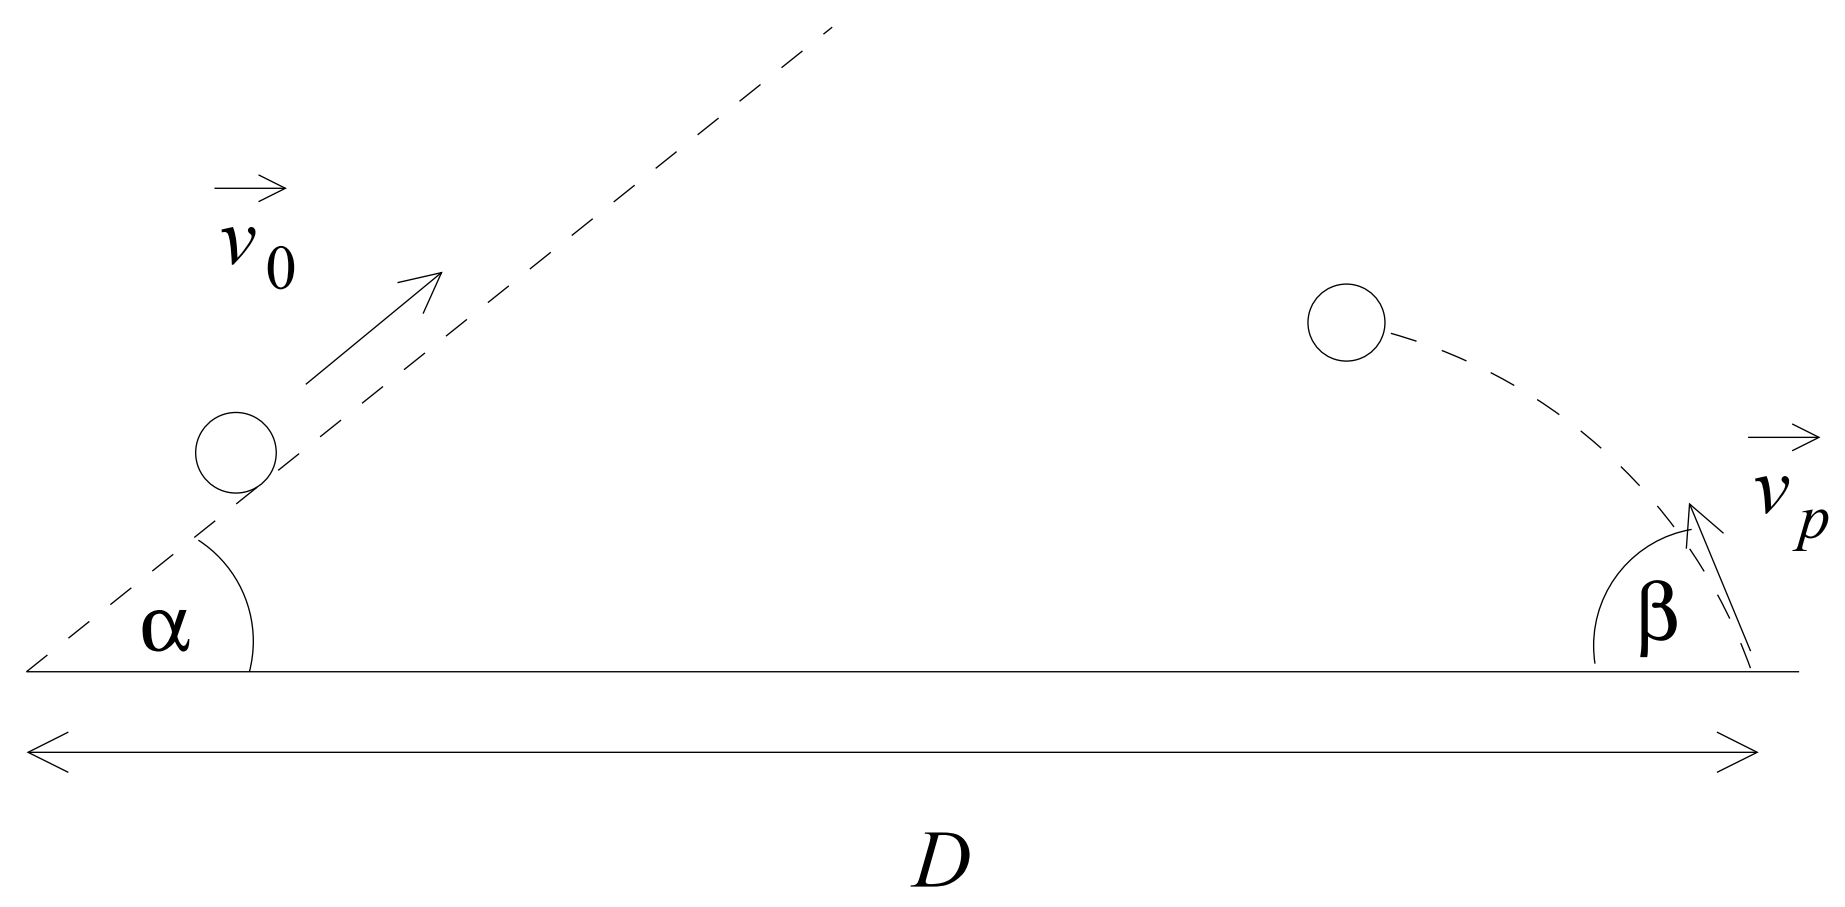
\includegraphics[width=0.86\linewidth]{2022-1/img/aux2/colision.PNG}
        \caption*{Fig. P3}
    \end{subfigure}
    \hspace{0.5cm}
    \begin{subfigure}[t]{0.4\textwidth}
        \centering
        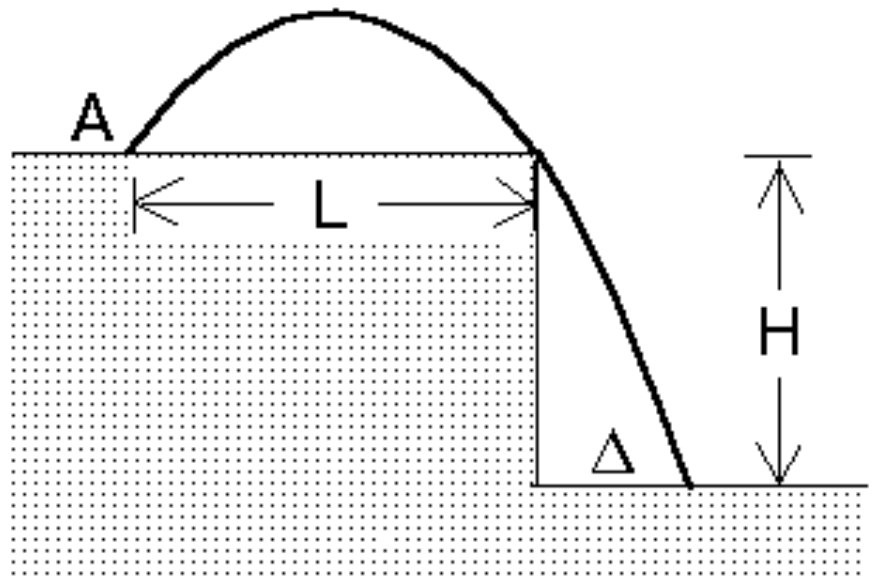
\includegraphics[width=0.6\linewidth]{2022-1/img/aux2/peldanio.PNG}
        \caption*{Fig. P4}
    \end{subfigure}
\end{figure}


\item Determine la máxima distancia $\Delta$ que un objeto puede alejarse del borde de un peldaño para evitar ser alcanzado por los objetos lanzados con velocidad $v_0$ desde el punto $A$. La distancia desde $A$ al borde del peldaño es $L$ y la altura de este es $H$



% Para imágenes vectoriales -> el texto tiene que estar en LaTeX
% \begin{figure}[htbp]
%   \centering
%   \svgpath{../Imagenes/ejercicios}  -> .. irse pa'trás 
%   \includesvg{ej5.svg}
% \end{figure}

\end{enumerate}
\end{document}
